\newpage
\section{System Perspective}

%A description and illustration of the:

%  - Design and architecture of your _ITU-MiniTwit_ systems
%  - All dependencies of your _ITU-MiniTwit_ systems on all levels of abstraction and development stages.
%    - That is, list and briefly describe all technologies and tools you applied and depend on.
%  - Important interactions of subsystems
%  - Describe the current state of your systems, for example using results of static analysis and quality assessments.
%  - Finally, describe briefly, if the license that you have chosen for your project is actually compatible with the licenses of all your direct dependencies.

%Double check that for all the weekly tasks (those listed in the schedule) you include the corresponding information.

\subsection{Design and architecture}

The technologies we selected to recreate the legacy Flask application ITU-MiniTwit, were C\# with the ASP.NET Core framework for the server and Postgresql as the database. The decision to use ASP.NET Core was made based on the team's prior experience, which enabled us to re-implement the Flask application's features quickly. Another reason for our selection was that with the performance enhancements of .NET 7, this is a very well performing framework\footnote{14th in this benchmark: 
\url{https://www.techempower.com/benchmarks/\#section=data-r21}}. \textit{README.md} in our GitHub repository contains instructions on how to run and deploy the system.
%This can also be seen in our group's solution being one of the top performing in this chart: \url{http://104.248.134.203/chart.svg}.

Figure \ref{fig:miniTwitApiOverview} shows the internal design of the MiniTwit application. We used Razor pages to render the web pages on the server side. For the course simulator to send request to our system we created an API at \textit{/simulator}.
%Over four weeks, the simulator provided our system with over 4 million messages/posts and nearly 13 million API calls.

\begin{figure}[H]
    \centering
    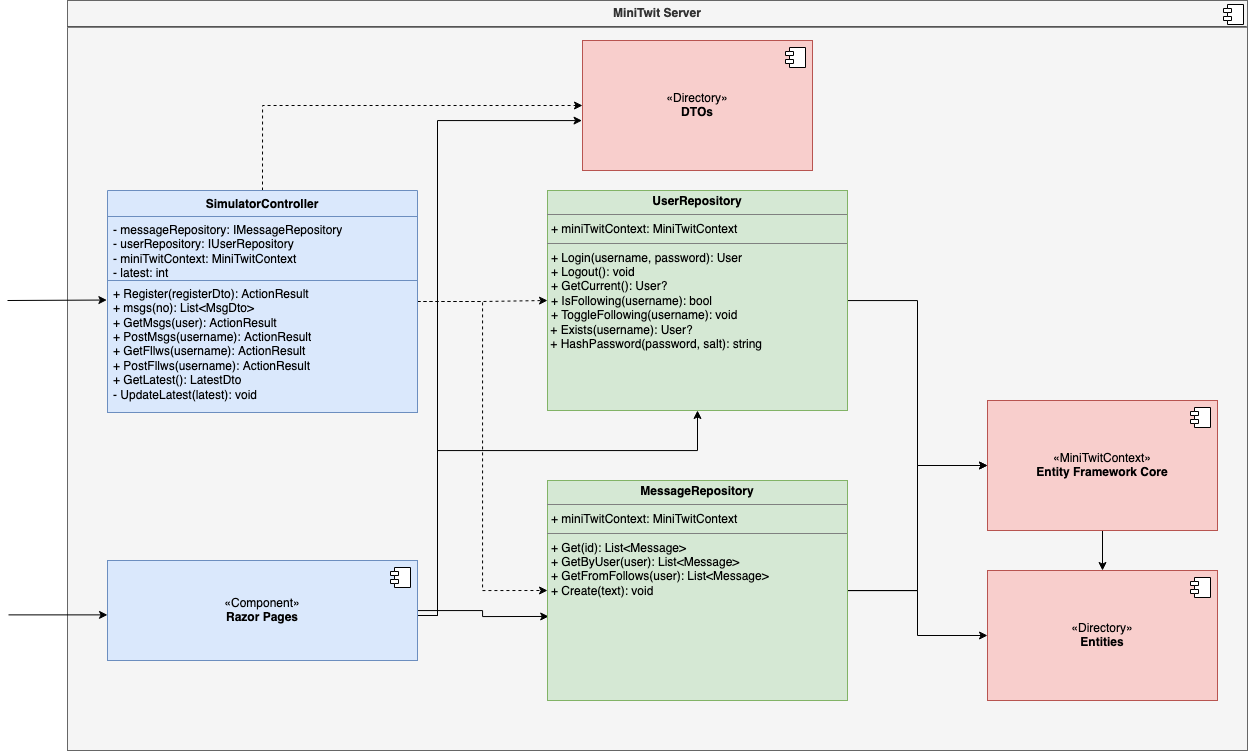
\includegraphics[width=\textwidth]{images/miniTwitServerOverview.png}
    \caption{Design of the MiniTwit service.}
    \label{fig:miniTwitApiOverview}
\end{figure}

Figure \ref{fig:architecture} shows the architecture of the final version of the system that was deployed, using three droplets (virtual machines) on DigitalOcean. Docker containers are within a docker swarm consitsting of one manager and two workers. There are three replicas of the MiniTwit server in the swarm, one on each droplet, to ensure availability. The two worker nodes only contain an instance of the MiniTwit server, while the manager includes load balancing, logging, and monitoring services. We decided to keep all these services on the same node to be accessible on the same IP address. Nginx is used for load balancing between the MiniTwit instances. Rolling updates are implemented through the docker swarm.

The database was hosted as a DigitalOcean managed database so that it was guaranteed to be reliable. Initially, we managed the Postgres database ourselves. However, one day, it suddenly crashed, which caused approximately 12 hours of downtime. We decided to switch to a managed database in our deployment to avoid worrying about this.

\begin{figure}[H]
    \centering
    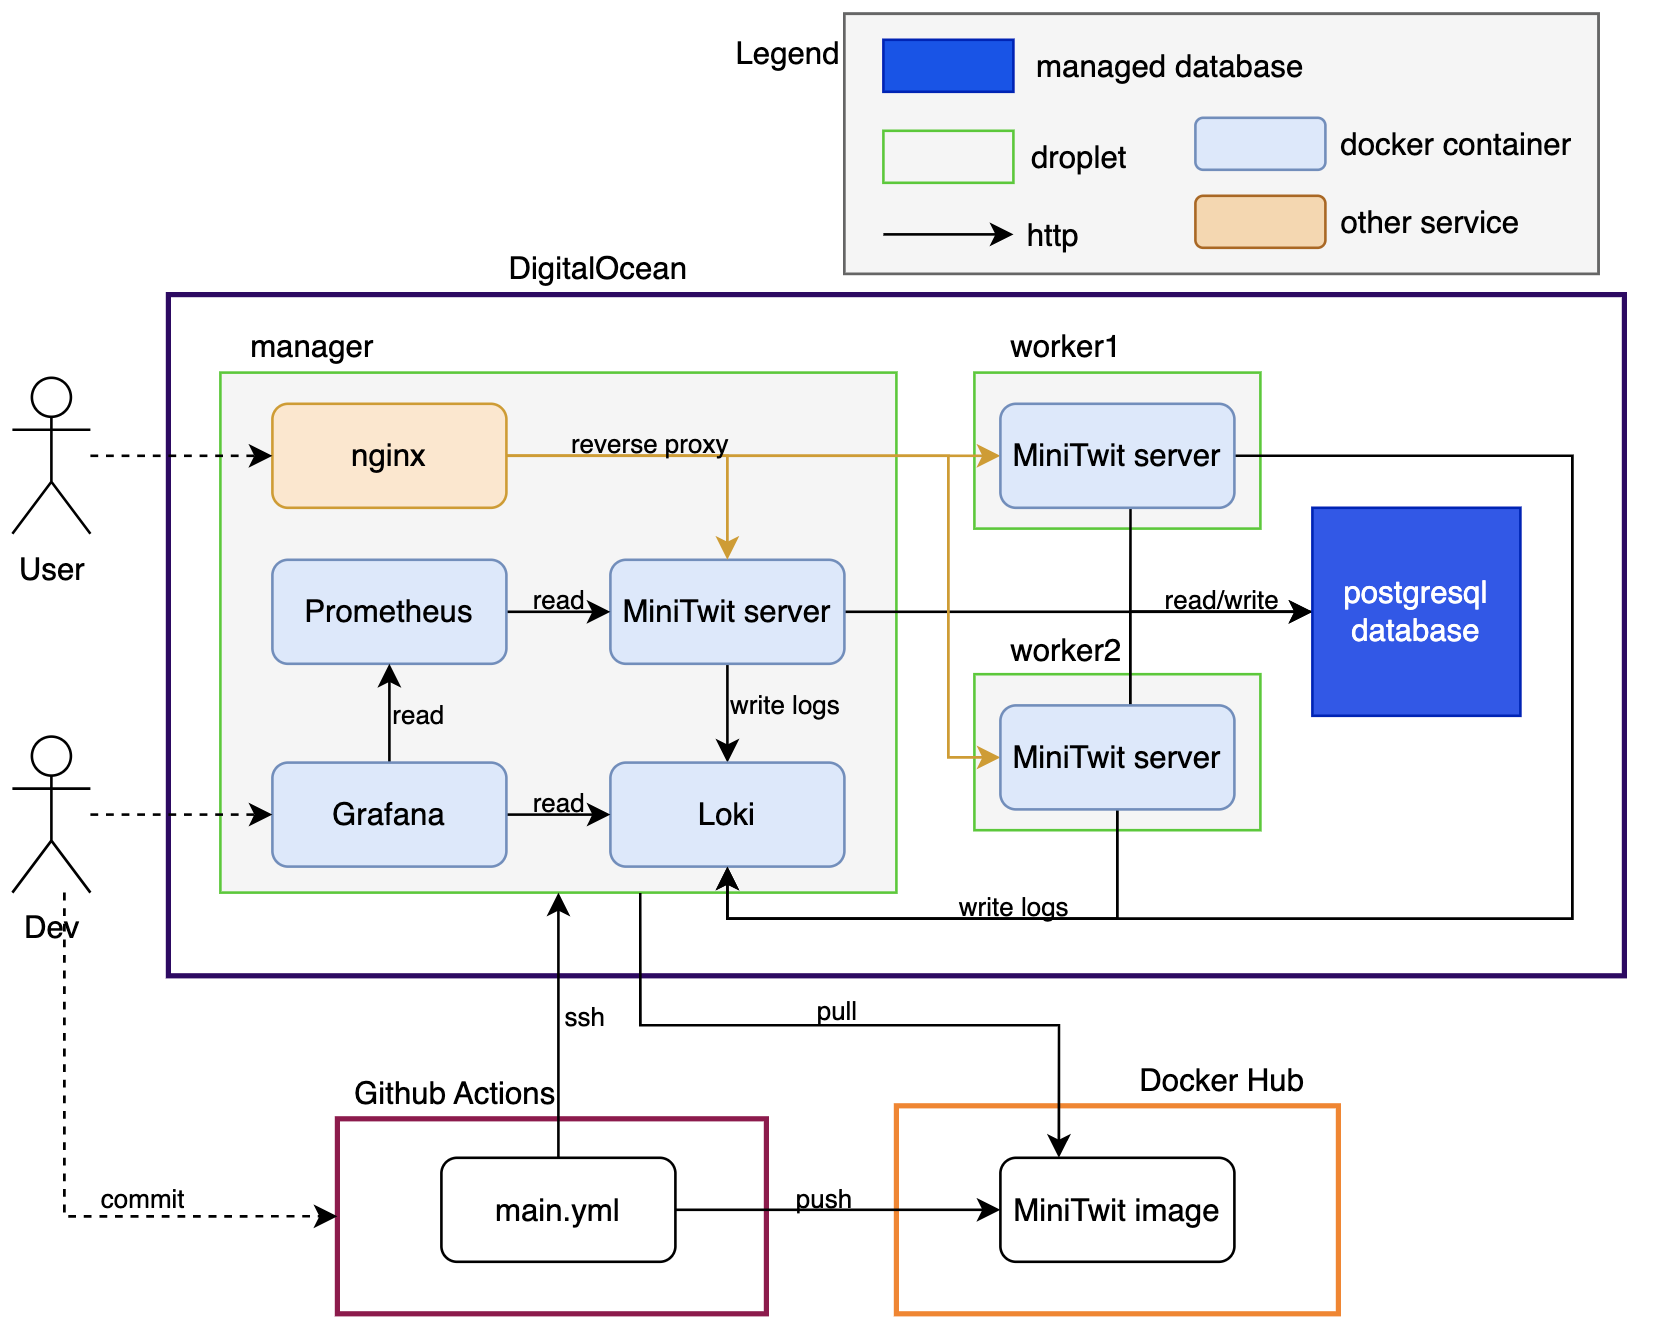
\includegraphics[width=\textwidth]{images/architecture2.png}
    \caption{Architecture of all subsystems in the final system.}
    \label{fig:architecture}
\end{figure}

\subsection{Technologies and Dependencies}

The technologies the system uses and depends on are listed below. All versions used were the most recent stable releases as of the start of 2023:

\begin{itemize}
    \item \textbf{ASP.NET Core}, for the web application.
    \item \textbf{PostgreSQL}, for data storage.
    \item \textbf{nginx}, for reverse proxy and load balancing.
    \item \textbf{Grafana}, for viewing metrics and logs.
    \item \textbf{Loki}, for storing logs.
    \item \textbf{Prometheus}, for storing metrics.
    \item \textbf{Docker}, for containerization.
    \item \textbf{Docker Hub}, for container image registry.
    \item \textbf{Ubuntu}, for the server OS.
    \item \textbf{Python}, for the tests.
    \item \textbf{Nuget}, for package management.
    \item \textbf{Github Actions}, for CI/CD.
    \item \textbf{DigitalOcean}, for infrastructure.
    \item \textbf{SonarCloud}, for static analysis.
    \item \textbf{Snyk}, for security assessments. \\
\end{itemize}

\noindent The libraries which the ASP.NET Core MiniTwit application depends on are:

\begin{outline}
    \1 \textbf{Entity Framework Core}, library for database abstraction layer.
    \1 \textbf{Npgsql}, library for connecting to Postgres from .NET.
    \1 \textbf{Serilog}, library for logging.
    \1 \textbf{Serilog.Sinks.Grafana.Loki}, library for shipping logs to Loki.
    \1 \textbf{Prometheus-net}, library to instrument .NET code with Prometheus metrics.
    \1 \textbf{SignalR}, library for real-time communication between server and client.
    \1 \textbf{code-cracker}, library for analyzing code.
\end{outline}

\subsection{Important interactions of subsystems}

Figure \ref{fig:architecture} also shows the interactions of the subsystems. Docker containers communicate via the internal network within the swarm. A user accesses the system via the address of the Nginx load balancer which reverse proxies to one of the active MiniTwit servers. The logging libraries we have used allows our MiniTwit servers ship logs itself, avoiding the need to have a log shipper instance, such as Promtail, on every node in the swarm.

A limitation of our chosen architecture is that Prometheus only reads from one of the MiniTwit server instances, the one on the same node. Since the load is balanced, only 1/3 of the traffic is monitored by metrics, and visible in Grafana. A similar problem appeared with the real-time updates we implemented with SignalR. Because of the load balancing, only every third message will, on average, appear for the user without reloading the page.

\subsection{Current state of systems}
Due to our project utilizing infrastructure as code, it is possible to turn the system on/off quickly. We have created a script, \textit{infrastructure.sh}, which deploys the entire system and provisions the infrastructure on DigitalOcean. When writing this report, we have turned the system off to minimize payments to Digital Ocean. When turning our system on, everything works as expected. The current code quality can be seen on our SonarQube page, which is showcased in figure \ref{fig:sonarQubeOverview}.

\begin{figure}[H]
    \centering
    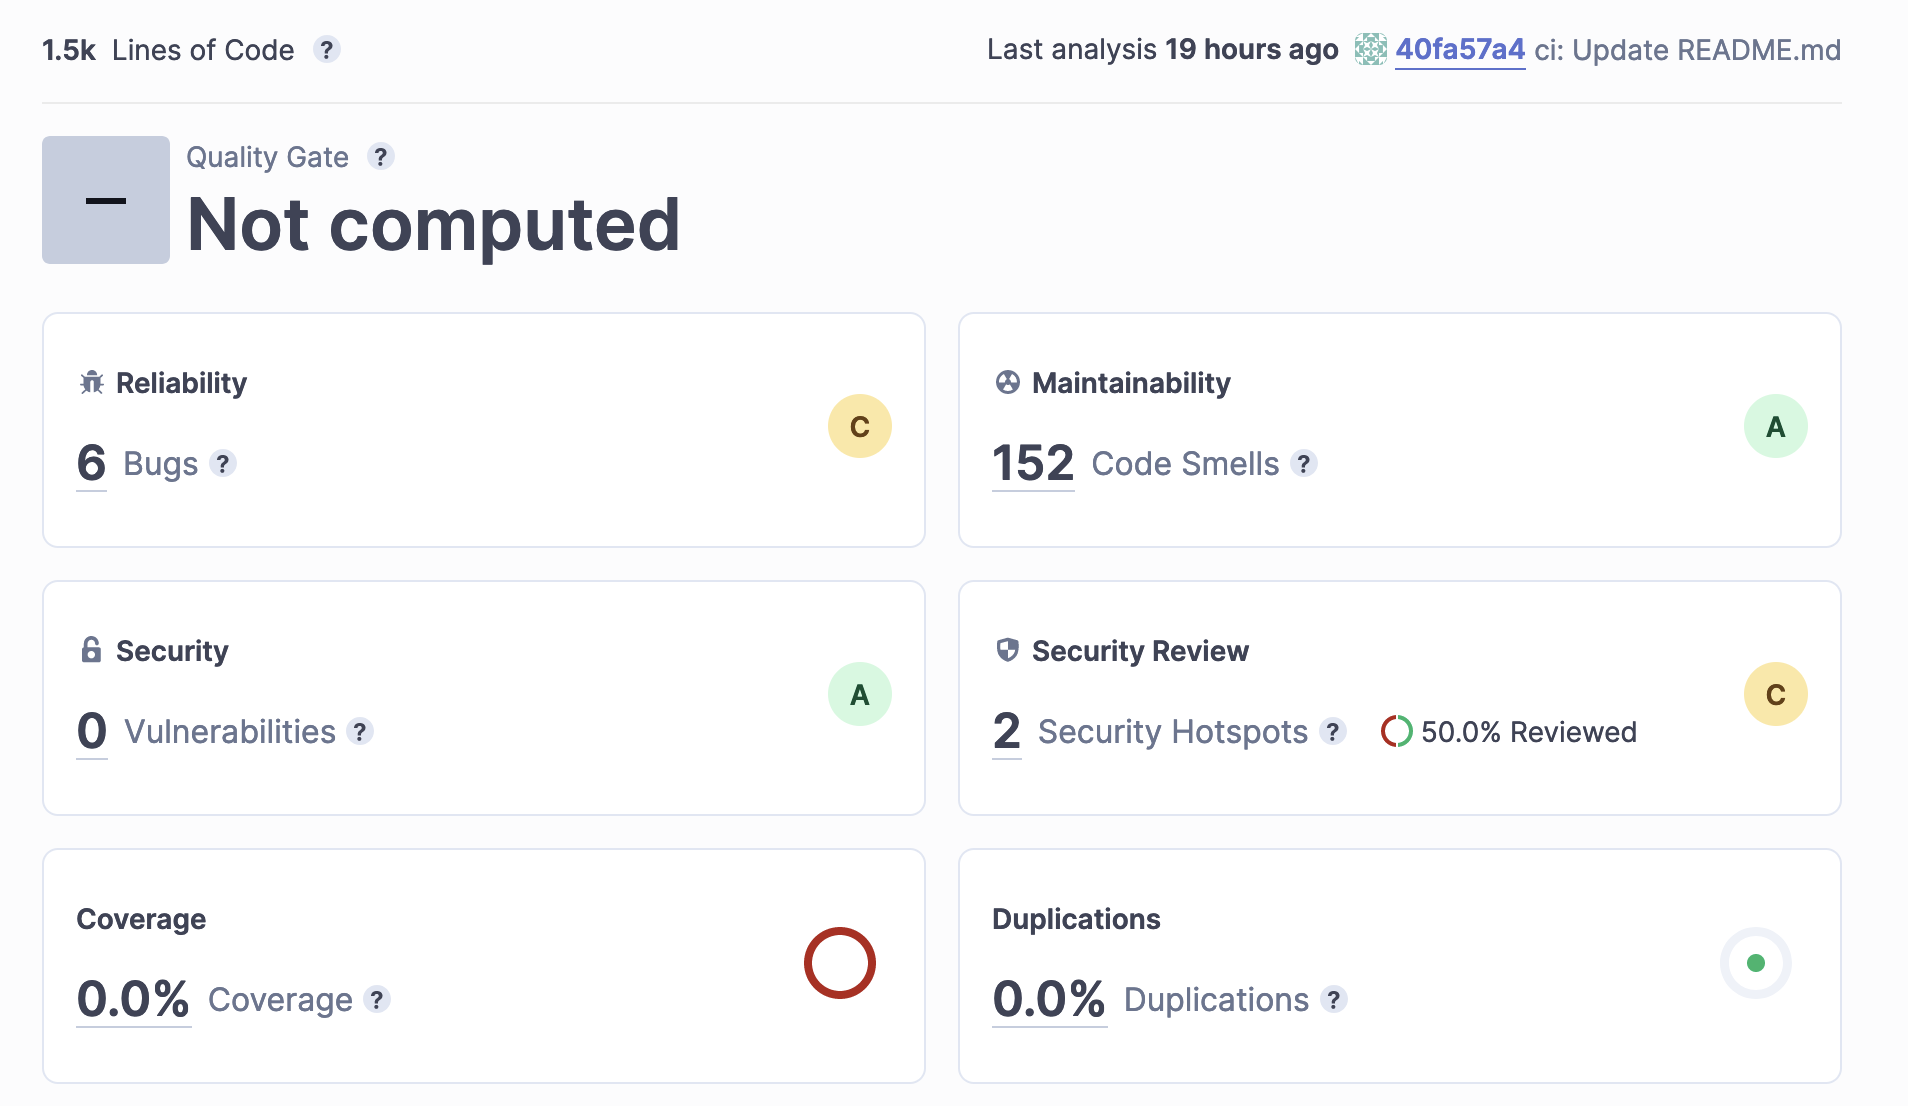
\includegraphics[width=\textwidth]{images/sonarStats.png}
    \caption{An overview of the code quality of the project in SonarQube.}
    \label{fig:sonarQubeOverview}
\end{figure}

%\todo[inline]{her kunne man lave sådan noget future work, altså hvis vi skulle arbejde videre på det hvad ville vi så lave?}

The current architecture and infrastructure comfortably handles the load of the simulator using three DigitalOcean droplets, which is likely overkill.

If we were to continue working on the system, a thing that we would work on is fixing the issues currently caused by having load balanced between multiple instances of the application server. Namely that 2/3 of metrics are not captured by Prometheus.
%For future work on the project, it would make sense to perfect the load-balancing aspect of the dockerized swarm. For example, the current setup means that Grafana only shows 1/3 of metrics, and when a user is connected to a MiniTwit server via WebSockets, this user would only receive 1/3 of new tweets. Currently, the WebSockets only send messages to clients when a change happens on the server instance, not when a change occurs in the database.

\subsection{License of our systems}
As we use the MIT license, and most of the direct dependencies use AGPLV3, we do not have any license conflicts. Our API also has an SLA.